\chapter{基于软硬协同的中断响应和任务调度设计}

在第二章中已经对任务模型以及相关的任务调度、I/O 模型等进行了详细的介绍,传统的进程、线程、协程模型是针对内核或者用户程序的各个功能单元来进行建模的,系统通过对这些任务对应的任务控制块进行管理,来实现任务的调度、同步、通信等功能,因此这些模型包含了任务生命周期内的所有相关的执行流(不仅包括在用户态运行的由应用程序定义的执行流,还包括了运行在内核中用于提供系统服务、中断处理以及异常处理的执行流),但这带来了以下问题:

\begin{itemize}
    \item 无法描述边界代码:在尚未完成任务管理模块初始化时,系统执行的初始化代码无法划分到其中的某个模型的实例中,在任务管理模块初始化之后,才划分到某个实例中。
    
    \item 无法描述中断处理例程:当 CPU 收到中断信号后,硬件保存部分现场,并暂停当前正在执行的任务,软件将剩下的寄存器现场保存在被暂停任务使用的栈上,紧接着复用被暂停任务的使用的栈跳转至中断处理例程,来完成中断信号的处理。在完成中断处理后,返回到被暂停的任务继续执行或者切换到新的任务。尽管在处理的过程中,当前正在运行的任务记录没有改变,且中断处理例程复用了当前被打断任务的栈,但它的功能不属于当前被打断的任务需要负责的功能单元,因此中断处理例程是无法归类到这些模型中的。由于中断处理例程的时间过长会严重影响系统的性能,Linux 内核将中断处理划分为上半段和下半段,上半段为一些必须紧急处理的事项(例如将设备的中断寄存器清空,完成必要的数据拷贝操作等);下半段则转化为一个单独的任务(例如网络协议处理等)。但这种将中断处理划分上下半段的方式仍然无法用传统的任务模型来描述上半段。如果使用单独的任务控制块来描述中断处理例程,这会增加系统的复杂性与开销,因为中断处理例程使用单独的栈来保存自己的状态,这会增加额外的任务切换开销,让中断响应延时(从中断触发产生到中断函数执行的时间)增加,并且由于需要为每个中断都需要准备额外的中断任务栈,无法应对中断嵌套的情况,在多核环境下,每个 CPU 都需要为同一个中断准备一个单独的中断任务栈,导致内存占用增大。
        
    \item 执行流之间的通信繁琐:由于内核只能对任务在内核中的执行流进行感知,用户态的执行流的变化无法被感知,因此导致了用户态的执行流无法直接与内核态的执行流进行通信,增加了通信的开销。在上一章节中对 I/O 模型的介绍详细描述了这个问题。(1)当用户态的执行流通过系统调用切换到内核执行流,若内核执行流阻塞,用户态的其他执行流将无法继续运行(同步阻塞 I/O 模型),内核执行流无法通知其他用户态执行流继续运行;(2)若内核执行流返回 \verb|EWOULDBLOCK| 通知其他用户态执行流可以继续执行,则增加了额外的轮询开销(同步非阻塞 I/O 模型);(3)在 I/O 多路复用模型中,内核执行流需要额外的机制(文件描述符集合的管理、事件循环等)来维护用户态执行流与 I/O 的状态信息;(4)基于信号或基于线程的回调函数构建的异步 I/O 模型增加了特权级切换的开销。
    
\end{itemize}

这些问题的核心在于任务模型的抽象粒度过大,需要将任务模型的粒度更加细化,并且需要打通执行流之间的通信壁垒。为此,本文提出了一种更细粒度的任务模型——基于执行流的任务模型。基于这种细粒度模型以及“\textbf{任务通信}”的视角,本文从以下方面展开对系统性能的优化:
\begin{itemize}
    \item 任务本身的开销;
    \item 任务切换的开销;
    \item 任务之间的通信开销;
\end{itemize}

针对系统中实现一定功能的普通任务的优化收益甚小,因此本文将优化的目标定为“中断处理”这个特殊的任务以及任务切换和任务之间的通信开销,设计了一套软硬协同的中断处理和任务调度机制,将中断处理任务和任务调度卸载到硬件中,减小了任务切换过程中调度的开销以及中断处理的开销,同时在硬件中搭建了任务之间的通信桥梁,减小任务的通信开销,并且提供了软硬件的交互接口。

\section{基于执行流的任务模型设计}

软件的执行流是指在 CPU 上执行的一段特定的功能单元,它既包含程序代码在运行过程中指令执行顺序和逻辑路径的动态描述(如顺序执行、条件分支、循环跳转等),也包含维持运行所需的独立资源环境(每个执行流属于某个操作系统或操作系统中的某个进程,运行于特定的特权级和地址空间中)。不同的执行流既能独立运行,也能通过通信协作完成特定功能。

本文基于软件执行流所处的独立资源环境(地址空间、特权级、堆栈)来构建任务模型,其中地址空间用来区分不同的操作系统或者操作系统中的进程,特权级用来区分用户态和内核态的执行流,堆栈用来保存执行流的函数调用关系等执行逻辑(线程模型)或状态(协程模型)\footnote{无栈协程使用有限状态机来表示内部的执行逻辑。}。因此,本文在保留进程概念的基础上(进程用于区分地址空间)使用 $T_{(P_{i}, L_{j}, S_{k})}$ 来符号化标识某个执行流的具体实例,其中:

\begin{itemize}
    \item $P_{i}$:表示执行流所处的进程(地址空间),$P_{i}$ 可以是内核,也可以是某个进程;
    \item $L_{j}$:表示执行流运行的特权级,$L_{j}$ 可以是用户态、内核态或其他特权级;
    \item $S_{k}$:表示执行流使用的堆栈;
\end{itemize}

由于这种任务模型的设计,任务之间的边界更加清晰,应用程序的逻辑由 $N$ 条在用户态运行的执行流与 $M$ 条在内核中运行的执行流共同组成,每个执行流构成独立的任务单元,任务之间的切换可以使用三元组($[prev]\longrightarrow [next] : \{condition\}$)进行描述,其中 $prev$、$next$ 分别表示切换前后的任务,$condition$ 表示切换的条件,可以是时间片耗尽、事件触发、系统调用等。典型的任务切换\footnote{在任务切换过程中,切换代码本身属于一段特殊的代码,它与任务本身的功能逻辑无关,但隶属于每个任务,当任务运行到切换代码时,切换代码即属于那个任务。}如下:

\begin{itemize}
    \item 相同地址空间内不跨越特权级的切换:
    \begin{equation*}
        T_{(P_{i}, L_{j}, S_{k})} \longrightarrow T_{(P_{i}, L_{j}, S_{l})} : \{\text{调度 | 内核态收到中断}\}
    \end{equation*}
    包括了分别在用户态/内核态由于调度引起的任务切换,这种切换只需要根据堆栈上保存的信息完成寄存器的上下文切换,因此开销较小。此外,无论是否使能 KPTI 机制,内核态任务所属的地址空间中均包含了内核地址空间的映射,因此在内核的任务收到中断信号后,不需要切换地址空间也不需要切换特权级,尽管复用了被暂停任务的栈,但栈上没有保存与中断处理任务相关的信息,因此可以认为切换了堆栈,所以这种切换属于第一类切换。

    \item 相同地址空间内跨越特权级的切换:
    \begin{equation*}
        T_{(P_{i}, L_{j}, S_{k})} \longrightarrow T_{(P_{i}, L_{l}, S_{n})} : \{\text{系统调用 | 异常 | 中断}\}
    \end{equation*}
    在没有使能 KPTI 机制的情况下,进程地址空间中包含了内核地址空间的地址映射,因此用户态任务获取内核提供的服务不需要切换地址空间,只需要切换到内核态下的任务;同理,异常与中断处理也不需要切换地址空间;
    
    \item 跨越地址空间但不跨越特权级的切换:前一个任务与被调度的下一个任务属于不同的进程,这种切换必须在高特权级中才能进行。
    \begin{equation*}
        T_{(P_{i}, L_{j}, S_{k})} \longrightarrow T_{(P_{l}, L_{j}, S_{n})} : \{\text{内核态任务调度}\}
    \end{equation*}

    \item 跨越地址空间且跨越特权级的切换:因为需要跨越地址空间,需要先从相同地址空间中的低特权级态切换到高特权级态,才可以切换地址空间,因此这种情况属于上述的第二类切换与第三类切换的组合。当使能 KPTI 机制时,用户态的任务必须要先切换到内核态下,再切换到内核的地址空间中,才可以使用系统提供的服务。
\end{itemize}

通过这种细粒度的任务建模,传统的系统调用以及中断处理可以被视为“\textbf{任务通信}”。系统调用可以视为用户态的任务将系统调用相关的参数信息打包成消息,通过相关的指令传递给处于内核态的用于处理系统调用的任务,内核态的任务处理完成后将结果返回给用户态的任务。

中断处理从表象上看是中断处理任务与硬件设备之间的交互,但其本质仍然是中断处理任务与其他任务之间的通信。例如,当系统调用任务调用 \verb|sleep()| 函数时,它告知中断处理任务,它需要在一段时间后被唤醒,中断处理任务在接收到时钟中断后,唤醒这个系统调用任务,这一套通信的流程构成了内核中提供的 \verb|sleep()| 系统服务,同理其他的系统服务也可以通过这种通信机制来进行解释。

\section{基于软硬协同的中断响应和任务调度机制}

任务调度器需要根据任务的状态以及调度策略来决定任务所处的队列,并维持队列的偏序关系。通常,任务的状态被保存在任务控制块中的某个字段中,任务调度器对任务状态字段所在的位置进行读写操作实现对任务状态的管理,并根据任务的状态将任务插入到不同的任务队列中。这一系列行为要求任务调度器获取任务控制块的位置、状态字段在任务控制块的偏移、任务的优先级以及任务队列的位置等信息。因此,将任务调度从软件卸载到硬件中,需要让硬件能够感知任务的状态、优先级等信息,并且在硬件中维护若干个任务队列,从而实现硬件任务调度器。

中断处理任务的功能是根据收到的中断信号,找到对应的任务,修改任务状态,并将任务放入到正确的任务队列中,这一系列操作需要获取中断信号、任务的状态、优先级等信息,以及任务队列的位置。因此,将中断处理任务卸载到硬件中需要以实现硬件任务调度器为前提。因此,基于软硬协同的中断响应和任务调度机制包括以下几个方面:

\begin{enumerate}
    \item 建立软硬协同的任务状态模型,实现硬件任务调度器;
    \item 以硬件任务调度器为前提,实现硬件中断处理机制(中断响应);
    \item 基于硬件中断处理机制实现硬件支持的任务通信机制;
\end{enumerate}

\subsection{硬件任务调度器}

实现硬件任务调度器需要对传统的任务状态模型进行扩展,使得硬件能够识别并修改任务的状态,本文设计了基于软硬协同的任务状态模型,如图 \ref{figure:task_state} 所示。

\begin{figure}[htbp]
    \centering
    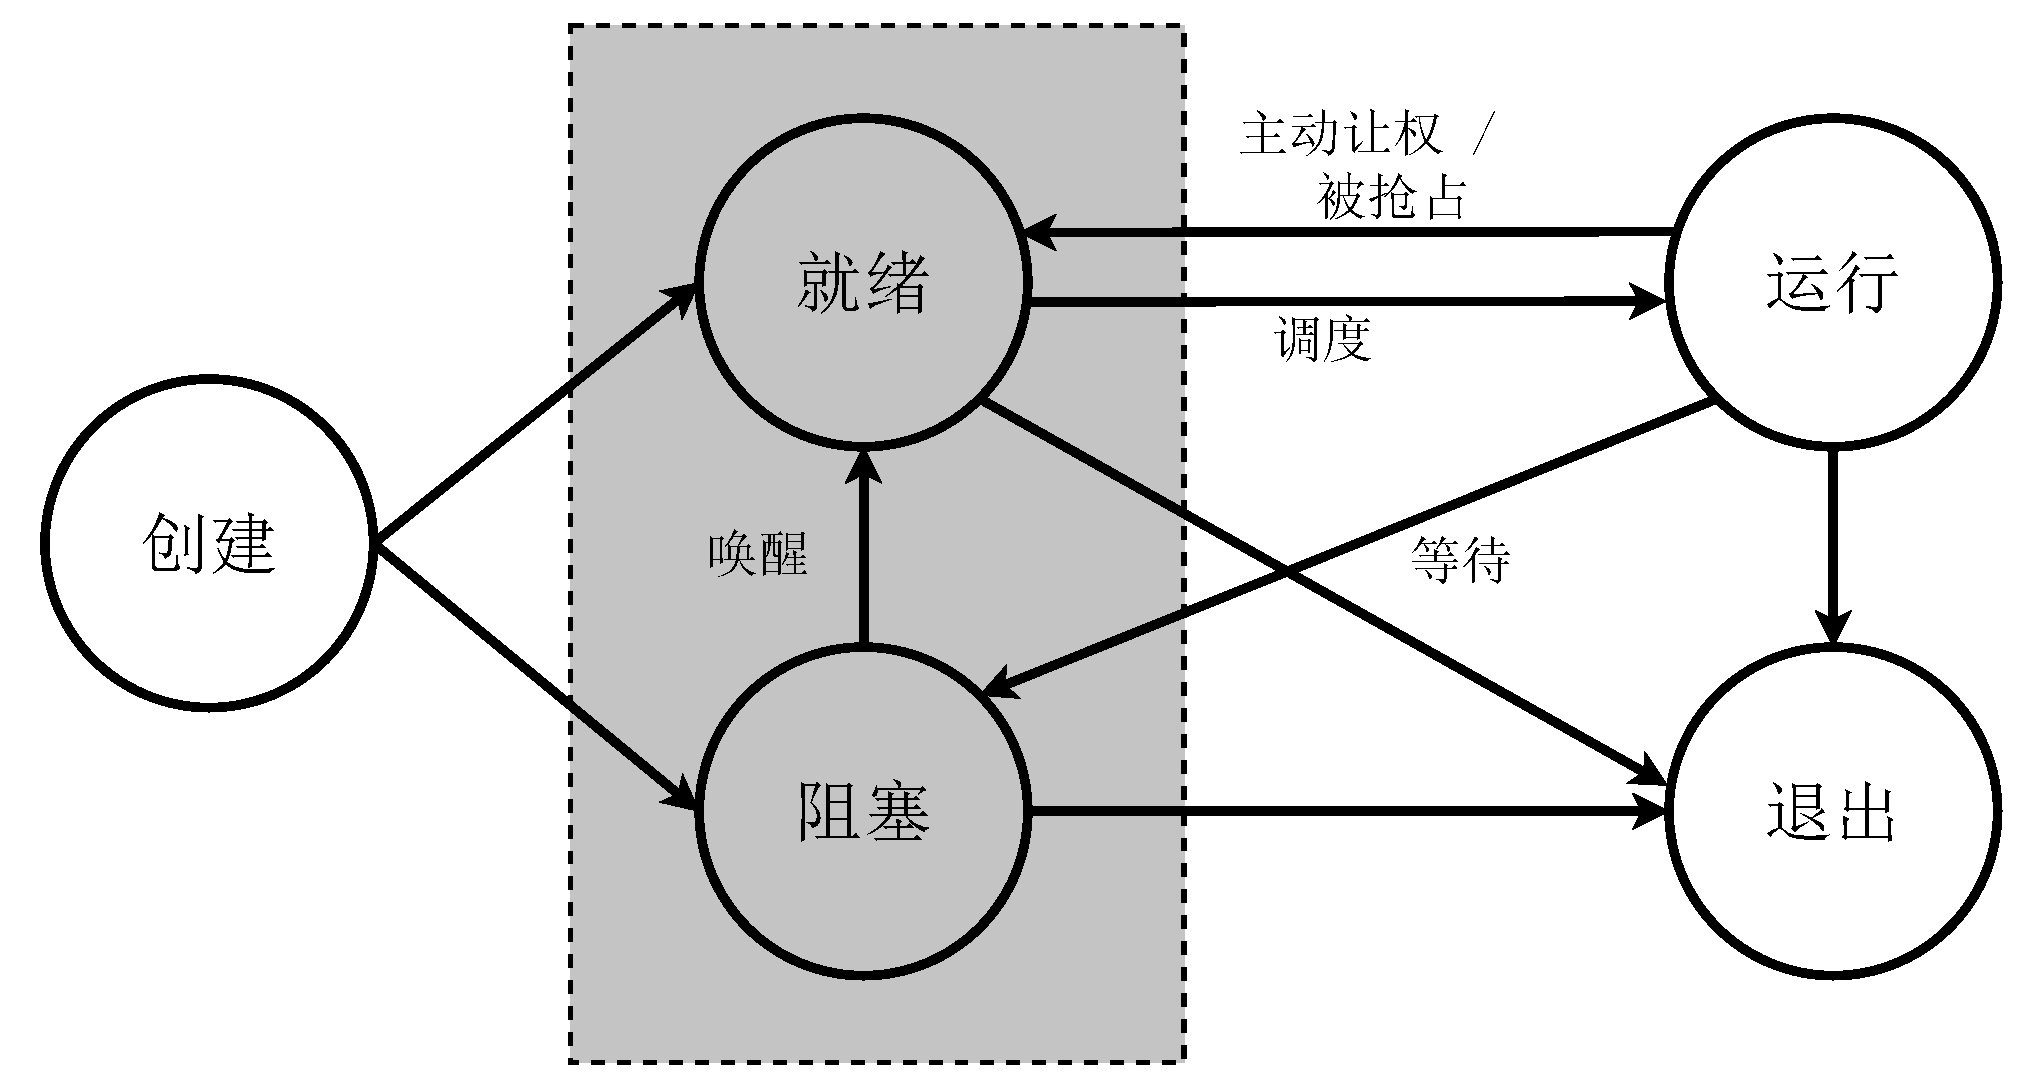
\includegraphics[width=0.8\textwidth]{figures/pdfs/task_state.pdf}
    \caption{基于软硬协同的任务状态模型}
    \label{figure:task_state}
\end{figure}

任务状态仍然为创建、就绪、运行、阻塞和退出这五种状态,其中灰色框线中的就绪态与阻塞态以及它们之间的状态转移由硬件任务调度器进行。硬件任务调度器在内部维护若干不同的就绪任务队列 $RQ_{*}$ 和阻塞任务队列 $BQ_{*}$,每个队列中存放任务的标识 $T_{(P_{i}, L_{j}, W_{k})}$(由任务的符号化标识 $T_{(P_{i}, L_{j}, S_{k})}$ 和任务的优先级 $W_{k}$ 等信息复合而成),并通过任务的优先级等信息维护任务队列的偏序关系。硬件调度器可以根据任务队列感知任务的状态以及优先级等信息,硬件通过将任务标识在这些队列中迁移实现对任务状态转移。硬件无法感知灰色框线外的其他任务状态,这些状态以及它们之间的转移由软件来维护,其他任务状态与就绪态、阻塞态之间的状态转移也由软件通过读写硬件调度器的响应端口来发起。任务的状态转移如下:

\begin{itemize}
    \item 创建 $\longrightarrow$ 就绪、创建 $\longrightarrow$ 阻塞:软件直接修改任务状态后,写硬件调度器的端口将创建的任务的标识添加至硬件调度器的就绪队列或者阻塞队列中;
    
    \item 就绪 $\longrightarrow$ 运行:软件读取硬件调度器的端口可以获取到就绪任务队列中最高优先级的任务标识,软件将任务的状态修改为运行态;
    
    \item 运行 $\longrightarrow$ 就绪:软件修改任务状态后,写硬件调度器的端口将任务标识添加至硬件调度器的就绪队列中;
    
    \item 运行 $\longrightarrow$ 阻塞:软件修改任务状态后,写硬件调度器的端口将任务标识添加至硬件调度器的阻塞队列中;
    
    \item 运行 $\longrightarrow$ 退出:软件直接修改任务状态;
    
    \item 阻塞 $\longrightarrow$ 就绪:硬件调度器根据特定的条件(例如收到中断信号)将阻塞队列中的任务标识添加至就绪队列中;这个过程硬件不直接修改任务状态,在软件从硬件调度器中取出就绪任务后,直接修改任务状态;
    
    \item 就绪 $\longrightarrow$ 退出、阻塞 $\longrightarrow$ 退出:软件向硬件调度器端口中写任务标识,硬件调度器将任务标识从就绪队列或阻塞队列中移除后,软件修改任务状态;
\end{itemize}

软件需要申请相应的就绪队列和阻塞队列,硬件任务调度器在成功分配了这些队列的硬件资源 $RQ_{(P_{i}, L{j})} + BQ_{(P_{i}, L{j})}$ 后,将会把这些队列相应的句柄(软件可以访问的硬件端口)返回给软件,软件通过该句柄来使用硬件任务调度器的功能。由于软件运行于一定的地址空间和特权级下(进程),在硬件队列申请成功后,直到进程生命周期结束或者软件主动释放掉硬件队列之前的这段时间,硬件队列与进程的地址空间 $P_{i}$ 和特权级 $L_{j}$ 相绑定。

使用硬件任务调度器,可以利用硬件机制来实现对任务队列的互斥访问,从而避免由于并发访问软件调度器带来的同步互斥开销。

\subsection{硬件中断处理机制}

\begin{figure}[htbp]
    \centering
    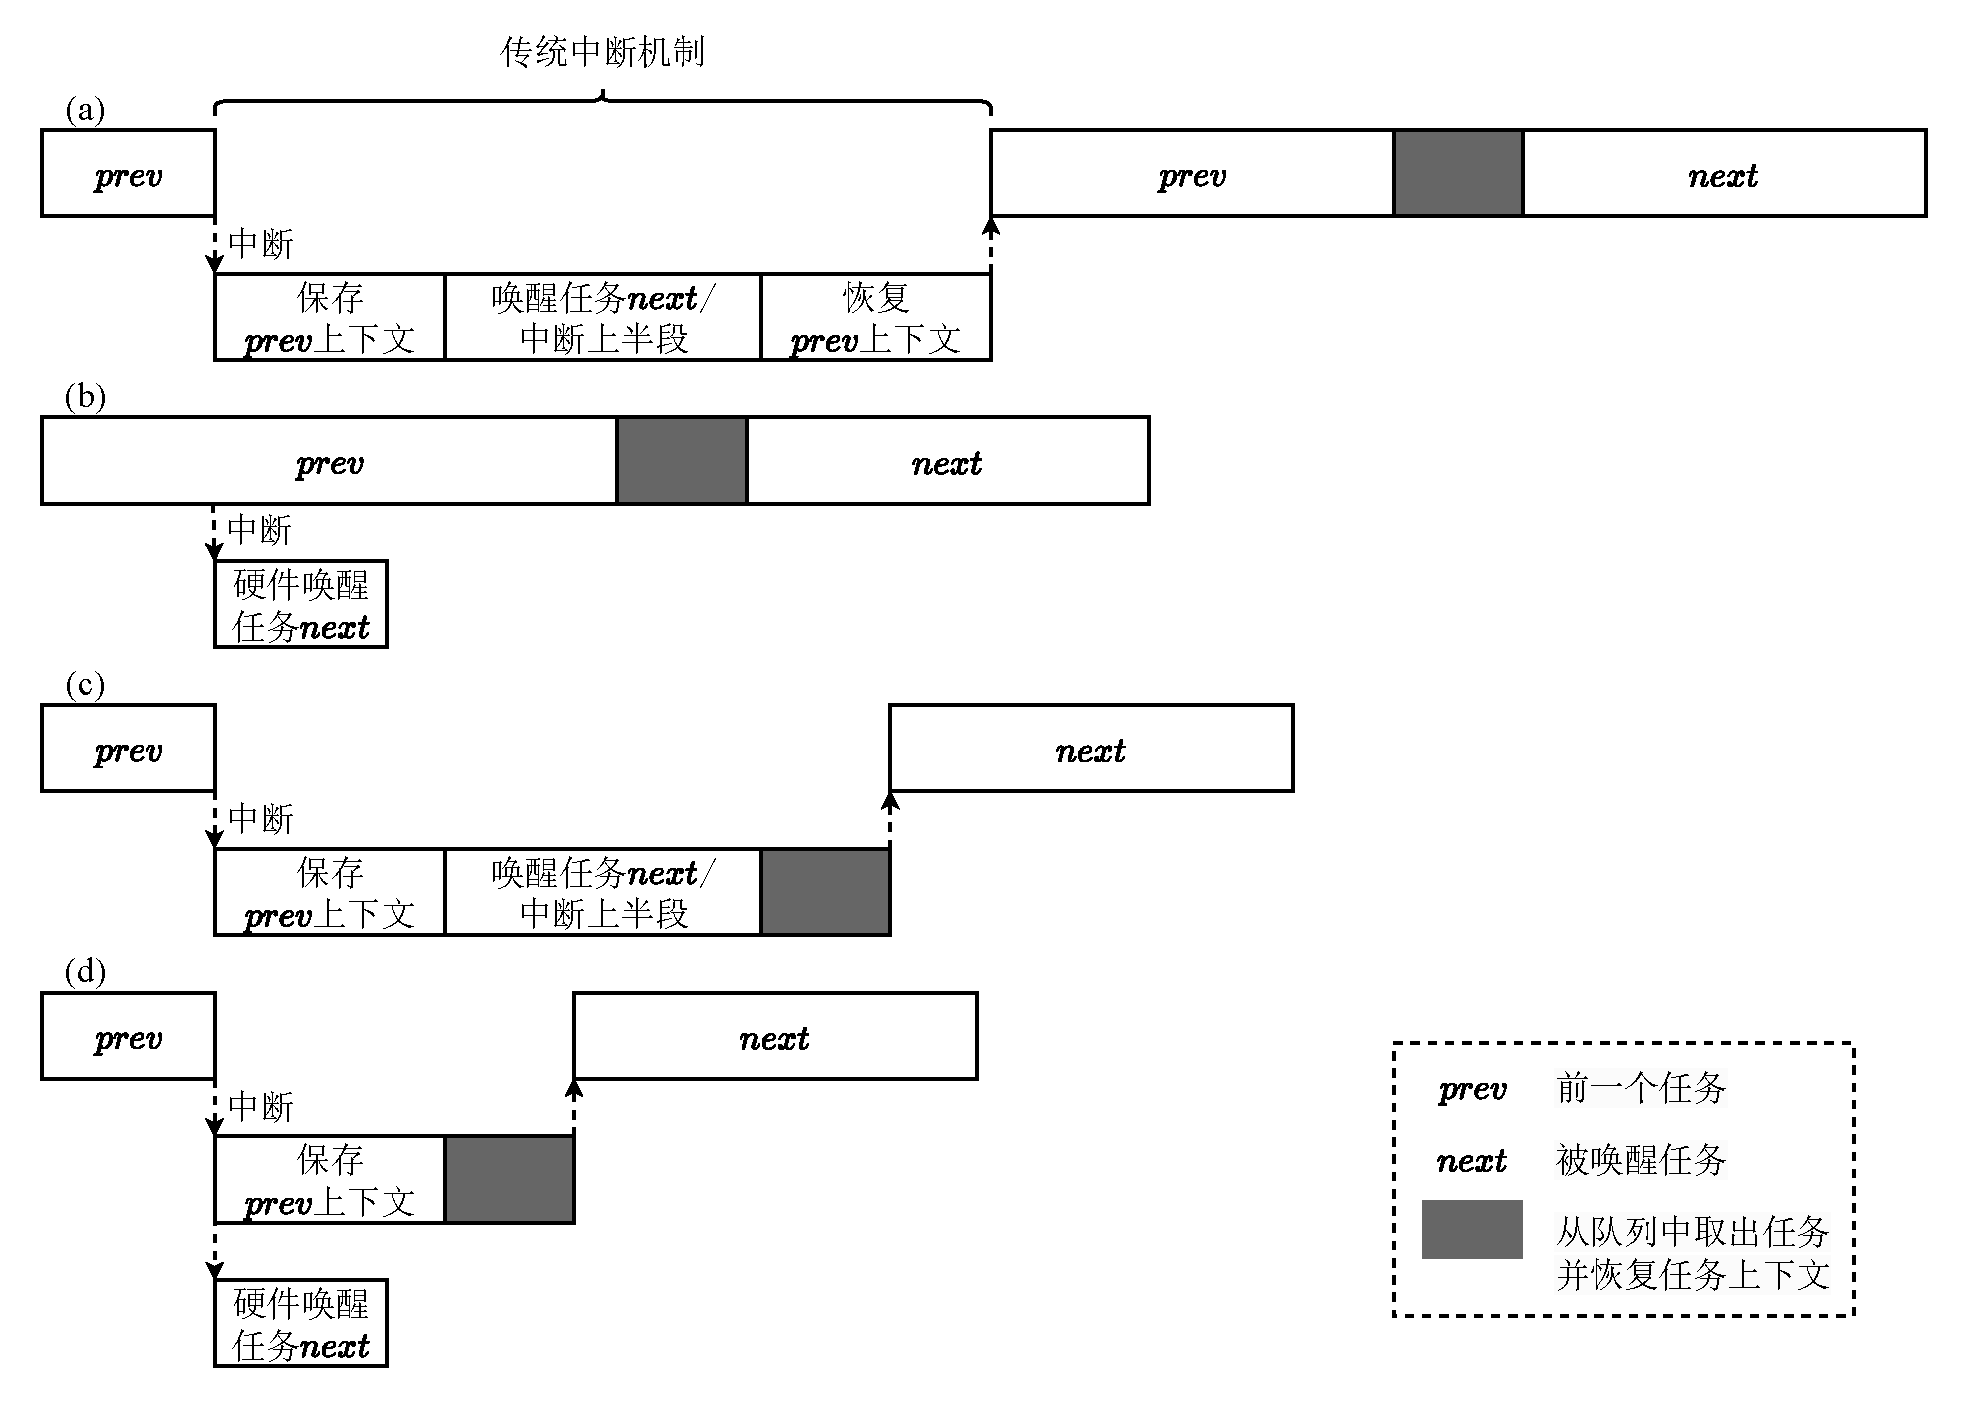
\includegraphics[width=\textwidth]{figures/pdfs/intr_demo.pdf}
    \caption{硬件处理中断图示,(a)为软件处理中断的流程,无任务抢占;(b)为硬件处理中断的流程,无任务抢占;(c)在(a)的基础上增加了任务抢占;(d)在(b)的基础上增加了任务抢占。}
    \label{figure:intr_demo}
\end{figure}

硬件中断处理机制的本质是用硬件电路来唤醒由于等待中断(I/O、定时器事件等)而进入阻塞状态的任务,这需要软硬件共同完成,其完整的流程如下:

\begin{enumerate}
    \item 软件向硬件调度器的端口中写任务标识,将其注册为某个中断信号的响应任务(硬件任务调度器将任务标识放入到与中断相关的阻塞队列中),预先将任务标识与中断进行绑定;
    \item 当硬件调度器收到中断信号后,根据中断信号的来源,找到对应的阻塞队列以及负责响应中断的任务标识,根据任务标识中的优先级信息,将任务标识从阻塞队列中移除,并放入到就绪队列中的合适位置;
    \item 如果唤醒的任务的优先级比当前正在 CPU 上运行的任务的优先级高,那么硬件任务调度器应该向 CPU 发送中断,CPU 在收到硬件任务调度器的中断信号后,直接进行任务切换。
\end{enumerate}

% \begin{figure}[htbp]
%     \centering
%     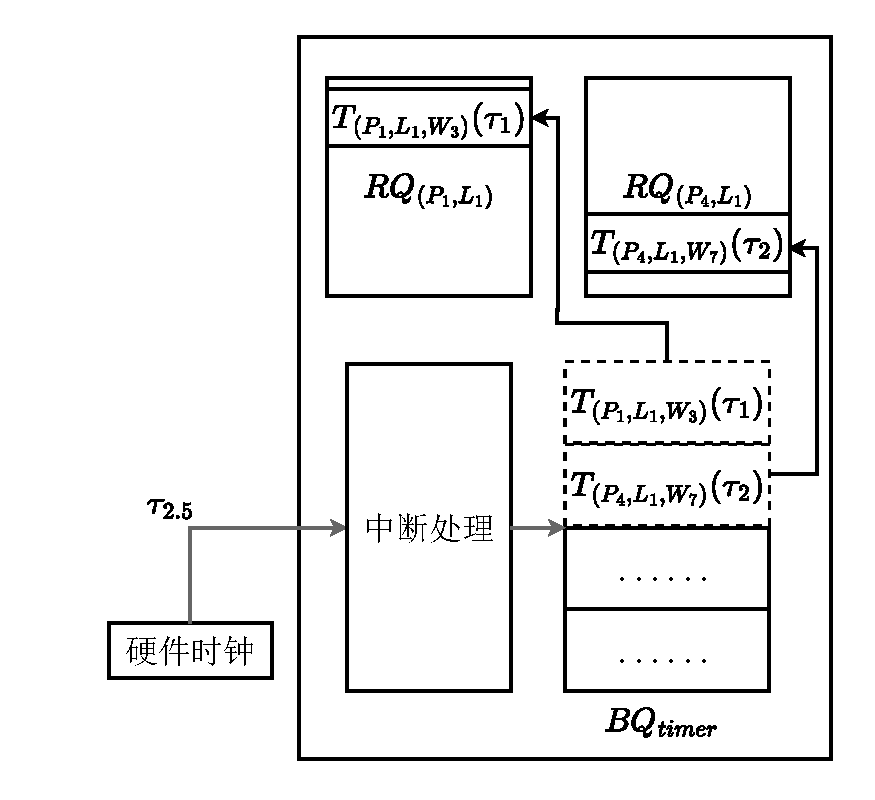
\includegraphics[width=0.8\textwidth]{figures/pdfs/timer.pdf}
%     \caption{硬件处理时钟中断}
%     \label{figure:timer}
% \end{figure}

% 以硬件处理时钟中断为例(如图 \ref{figure:timer}),硬件任务调度器在内部实现了与时钟中断相关的阻塞任务队列($BQ_{timer}$)来维护由于等待定时器事件而进入阻塞状态的任务标识($T_{(P_{i}, L_{j}, W_{k})}(\tau_{t})$,标识中增加了定时器的截止时间 $\tau_{t}$),该队列根据任务所等待的定时器的截止时间 $\tau_{t}$ 的先后顺序进行排序。在 $\tau_{2.5}$ 时刻,硬件时钟产生时钟中断,将信号发送给硬件任务调度器,硬件任务调度器检查 $BQ_{timer}$ 队列头部的任务所等待的定时器事件的截止时间,发现任务标识 $T_{(P_{1}, L_{1}, W_{3})}(\tau_{1})$ 和 $T_{(P_{4}, L_{1}, W_{7})}(\tau_{2})$ 的截止时间小于当前时间,因此,硬件任务调度器根据任务标识中的进程标识和特权级标识找到对应的就绪队列,并根据任务标识中的优先级信息将其放入到就绪队列的适当位置,完成硬件中断处理。

通过硬件快速响应中断,唤醒阻塞的任务,可以让 CPU 不被一些中断信号打断,减少由于中断导致的中断上下文切换开销。若被唤醒的任务优先级较高,需要进行任务切换,在这种情况下,仍然可以减少由于中断导致的调度开销,硬件中断处理机制与传统机制的对比如图 \ref{figure:intr_demo} 所示。

\subsection{硬件支持的任务通信机制}

通信中的两个任务分别为发送方与接收方,它们属于不同的地址空间或不同特权级下的进程。使用硬件支持的任务通信机制的前提是通信的双方都使用了硬件提供的任务调度器功能(双方进程分别使用不同的任务队列),并且,在上述的硬件中断处理机制的基础上,将中断信号的发送方从硬件设备扩展为软件上的发送方任务。此外,硬件中还需要维护与双方通信能力相关的能力槽,并配置额外的能力检查机制来避免恶意通信。其完整的通信流程如下:

\begin{enumerate}
    \item 发送方与接收方申请使用硬件任务调度器;

    \item 发送方任务向硬件任务调度器的端口中写接收方任务的进程标识以及中断号,硬件任务调度器将这两项信息填写至发送方的发送能力槽中,从而注册可以向指定接收方进程发送的指定中断的能力;
    
    \item 接收方任务向硬件任务调度器的端口中写发送方任务的进程标识、中断号以及自己的标识,硬件任务调度器将这些信息填写至接收方的接收能力槽中,从而注册可以接收指定发送方的指定中断的能力;
    
    \item 发送方任务向硬件任务调度器的端口中写接收方的进程标识以及中断号,尝试进行通信。硬件任务调度器首先检查发送方的发送能力槽中是否存在对应的接收方进程标识以及中断号。如果存在,则硬件任务调度器根据接收方的进程标识找到对应的接收方进程所使用的就绪队列以及接收能力槽,如果接收能力槽中存在对应的发送方的进程标识、中断号以及接收方的任务标识,则硬件任务调度器将接收方的任务标识放入到接收方的就绪队列中的适当位置,完成通信。

\end{enumerate}

基于硬件支持的通信机制,跨域不同地址空间和特权级的执行流之间可以实现快速交互,减少了切换地址空间以及特权级的开销,图展示了信号机制与使用 TAIC 机制进行通信的对比。

\begin{figure}
    \centering
    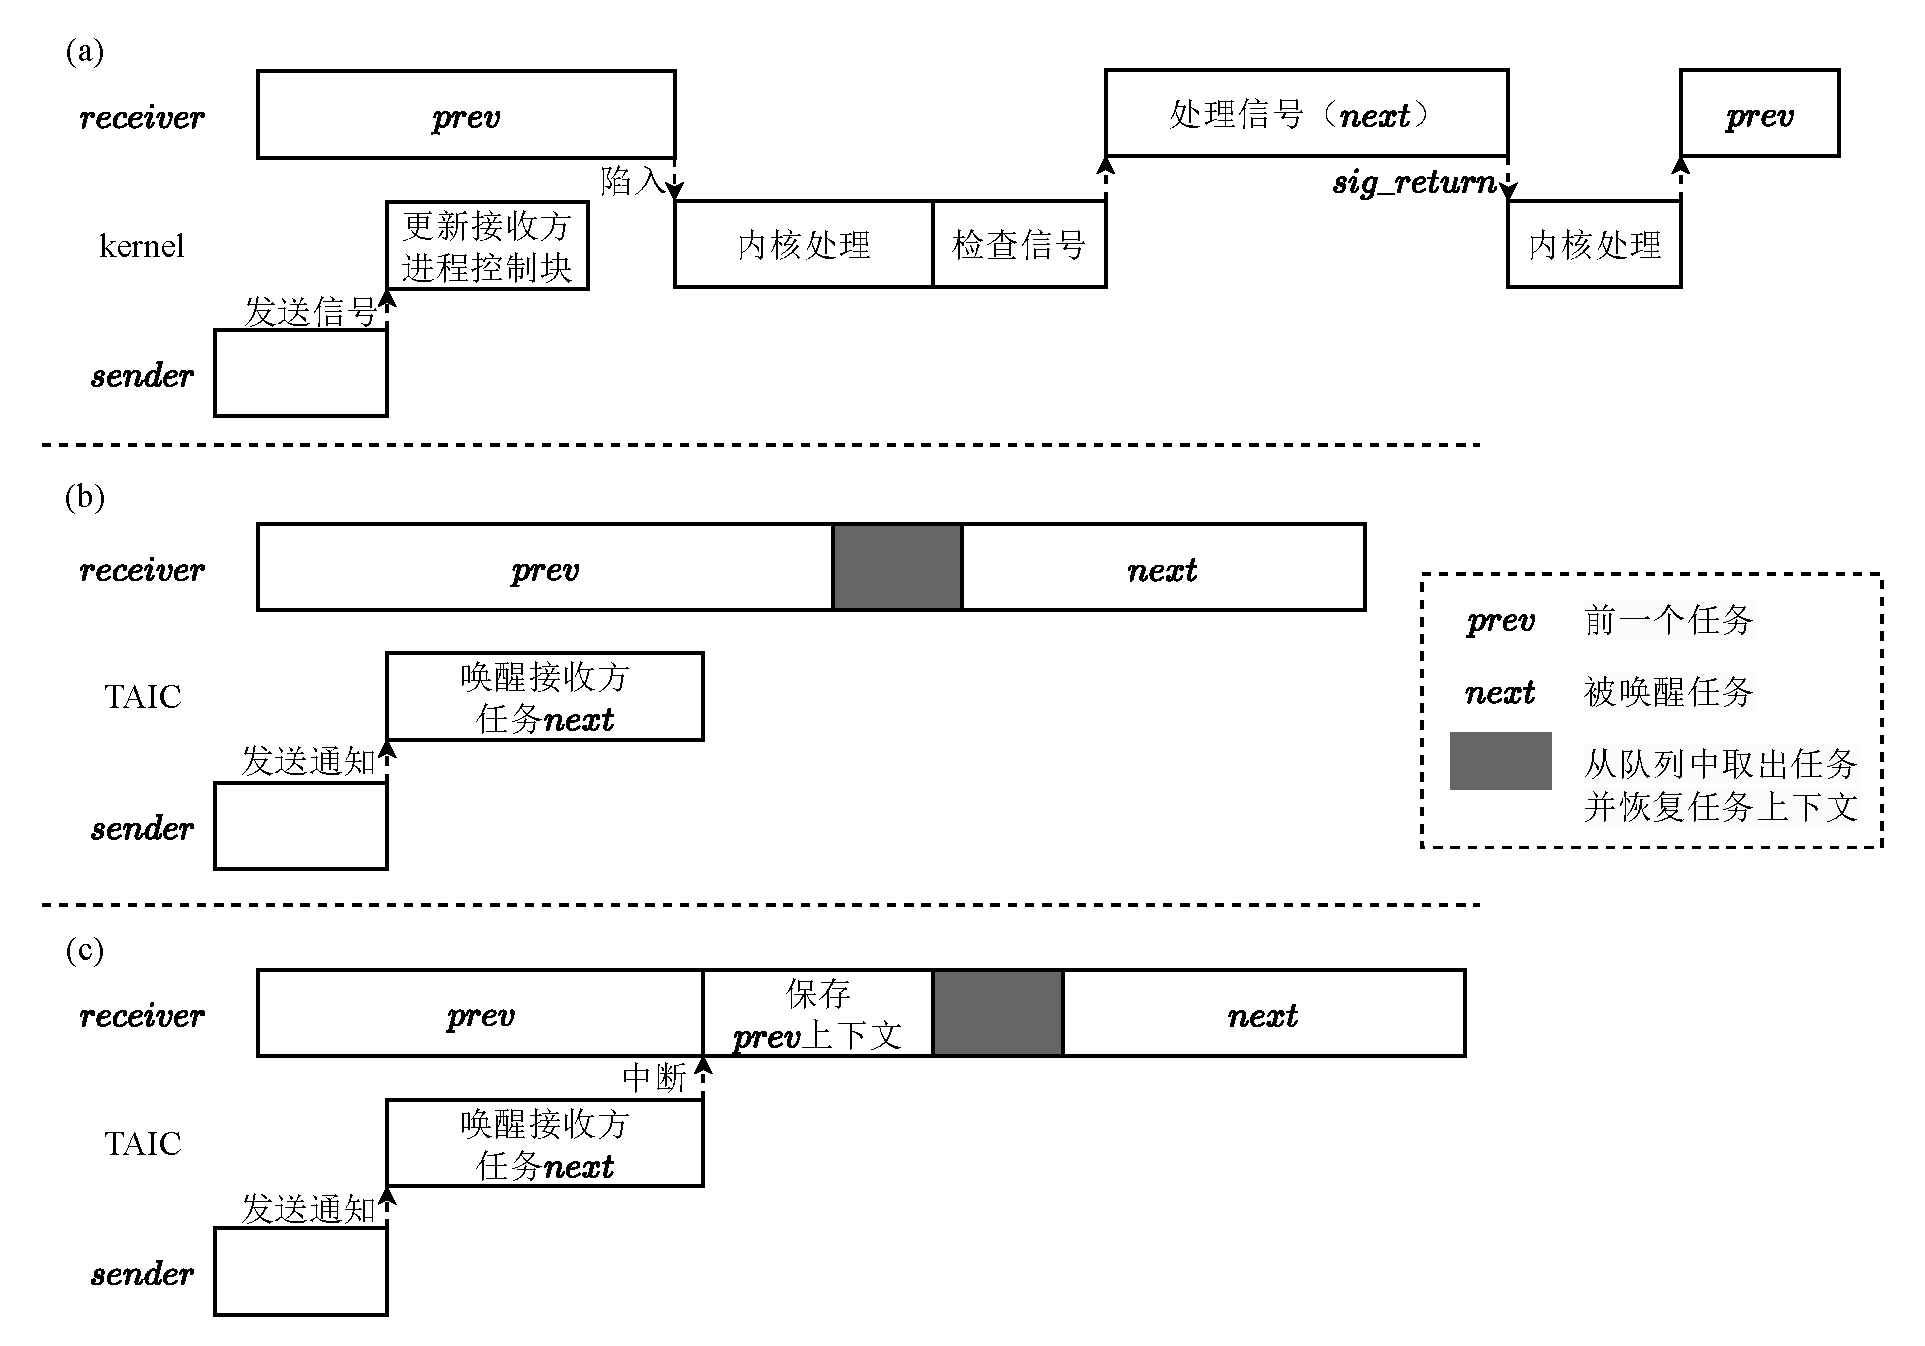
\includegraphics[width=\textwidth]{figures/pdfs/communicate_demo.pdf}
    \caption{IPC 对比,(a)为基于信号机制的通信流程;(b)为使用 TAIC 机制的通信流程,没有任务抢占;(c)在(b)的基础上增加了任务抢占。}
\end{figure}

\section{软硬件交互接口}

I/O 端口作为软件访问硬件的入口,也是硬件响应软件操作并返回结果的媒介。软件通过向 I/O 端口发送读写命令,将数据与控制信号传递给硬件,最终转化为对硬件中的寄存器或状态的操作,从而驱动硬件完成特定的功能。在本文的基于软硬协同的中断响应和任务调度机制中,软硬件相互协作,共同完成任务调度、中断处理以及任务通信等功能,软硬件之间的交互接口如表 \ref{table:io_interface} 所示。

\begin{table}[htbp]
    \centering
    \caption{软硬件交互接口}
    \label{table:io_interface}
    \begin{tabular}{lll}
        \toprule
        功能 & 接口 & 说明 \\
        \midrule
        \multirow{2}{*}{\makecell[l]{硬件资源 \\ 申请与回收}} & alloc & \makecell[l]{软件写端口,申请的队列资源,并从端口中读出 \\ 队列资源句柄} \\
        & free & \makecell[l]{软件写需要回收的句柄,硬件回收队列资源} \\ \hline
        \multirow{3}{*}{任务调度} & task\_enqueue & \makecell[l]{软件写任务标识,硬件将标识添加至就绪队列中} \\
        & task\_dequeue & \makecell[l]{软件从硬件中读出优先级最高的就绪任务标识} \\
        & remove\_task & \makecell[l]{软件写任务标识,硬件将删除队列中的任务标识} \\ \hline
        \multirow{2}{*}{外部中断处理} & register\_extint & \makecell[l]{软件写任务标识,将任务与中断绑定} \\
        & unregister\_extint & \makecell[l]{软件取消任务与中断之间的绑定} \\ \hline
        \multirow{5}{*}{任务通信} & register\_sender & \makecell[l]{软件写接收方进程标识和中断号,注册发送能力} \\
        & unregister\_sender & \makecell[l]{软件写接收方进程标识和中断号,取消发送能力} \\
        & register\_receiver & \makecell[l]{软件写发送方进程标识、中断号和接收方任务 \\ 标识,注册接收能力} \\
        & unregister\_receiver & \makecell[l]{软件写发送方进程标识和中断号,取消接收能力} \\
        & send & \makecell[l]{软件写接收方进程标识和中断号,发起通信} \\
        \bottomrule
    \end{tabular}
\end{table}

\section{本章小结}

本章提出基于执行流的任务模型,从“\textbf{任务通信}”的视角出发,将任务调度、中断处理以及任务通信组合成统一整体,利用硬件快速、高效等特点对其进行加速,设计了基于软硬协同的中断响应和任务调度机制,综合性地减小系统开销,提高系统应对应用场景复杂多样的性能需求。
